

\tikzset{every picture/.style={line width=0.75pt}} %set default line width to 0.75pt        

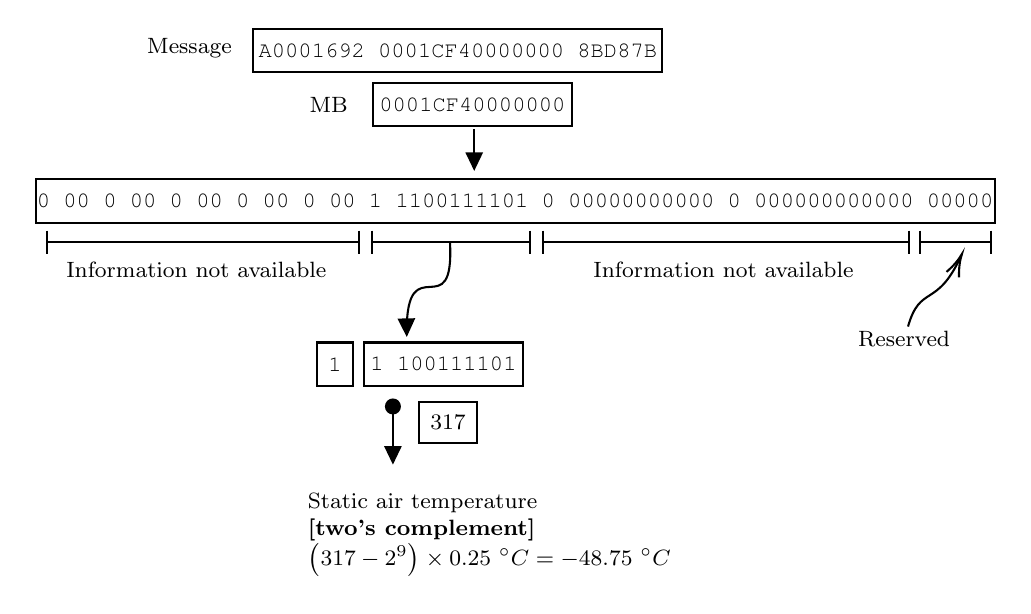
\begin{tikzpicture}[x=0.75pt,y=0.75pt,yscale=-1,xscale=1]
%uncomment if require: \path (0,368); %set diagram left start at 0, and has height of 368

%Straight Lines [id:da4065588661974868] 
\draw [line width=0.75]    (182.67,117.33) -- (259,117.33) ;
\draw [shift={(259,117.33)}, rotate = 180] [color={rgb, 255:red, 0; green, 0; blue, 0 }  ][line width=0.75]    (0,5.59) -- (0,-5.59)   ;
\draw [shift={(182.67,117.33)}, rotate = 180] [color={rgb, 255:red, 0; green, 0; blue, 0 }  ][line width=0.75]    (0,5.59) -- (0,-5.59)   ;
%Straight Lines [id:da8606101743392234] 
\draw [line width=0.75]    (265,117.33) -- (441.5,117.33) ;
\draw [shift={(441.5,117.33)}, rotate = 180] [color={rgb, 255:red, 0; green, 0; blue, 0 }  ][line width=0.75]    (0,5.59) -- (0,-5.59)   ;
\draw [shift={(265,117.33)}, rotate = 180] [color={rgb, 255:red, 0; green, 0; blue, 0 }  ][line width=0.75]    (0,5.59) -- (0,-5.59)   ;
%Curve Lines [id:da10322788127976112] 
\draw    (220.33,117.33) .. controls (222.46,159.15) and (199.45,118.69) .. (199.47,160.35) ;
\draw [shift={(199.5,163)}, rotate = 268.75] [fill={rgb, 255:red, 0; green, 0; blue, 0 }  ][line width=0.08]  [draw opacity=0] (8.93,-4.29) -- (0,0) -- (8.93,4.29) -- cycle    ;
%Straight Lines [id:da8466832782097071] 
\draw    (232,63) -- (232,80) ;
\draw [shift={(232,83)}, rotate = 270] [fill={rgb, 255:red, 0; green, 0; blue, 0 }  ][line width=0.08]  [draw opacity=0] (8.93,-4.29) -- (0,0) -- (8.93,4.29) -- cycle    ;
%Straight Lines [id:da4977418628626593] 
\draw    (192.83,196.5) -- (192.83,221.5) ;
\draw [shift={(192.83,224.5)}, rotate = 270] [fill={rgb, 255:red, 0; green, 0; blue, 0 }  ][line width=0.08]  [draw opacity=0] (8.93,-4.29) -- (0,0) -- (8.93,4.29) -- cycle    ;
\draw [shift={(192.83,196.5)}, rotate = 90] [color={rgb, 255:red, 0; green, 0; blue, 0 }  ][fill={rgb, 255:red, 0; green, 0; blue, 0 }  ][line width=0.75]      (0, 0) circle [x radius= 3.35, y radius= 3.35]   ;
%Straight Lines [id:da5955016490623266] 
\draw [line width=0.75]    (26,117.33) -- (176.5,117.33) ;
\draw [shift={(176.5,117.33)}, rotate = 180] [color={rgb, 255:red, 0; green, 0; blue, 0 }  ][line width=0.75]    (0,5.59) -- (0,-5.59)   ;
\draw [shift={(26,117.33)}, rotate = 180] [color={rgb, 255:red, 0; green, 0; blue, 0 }  ][line width=0.75]    (0,5.59) -- (0,-5.59)   ;
%Straight Lines [id:da5052935437984565] 
\draw [line width=0.75]    (446.67,117.33) -- (481,117.33) ;
\draw [shift={(481,117.33)}, rotate = 180] [color={rgb, 255:red, 0; green, 0; blue, 0 }  ][line width=0.75]    (0,5.59) -- (0,-5.59)   ;
\draw [shift={(446.67,117.33)}, rotate = 180] [color={rgb, 255:red, 0; green, 0; blue, 0 }  ][line width=0.75]    (0,5.59) -- (0,-5.59)   ;
%Curve Lines [id:da0284439343230396] 
\draw    (441,158) .. controls (446.88,137.42) and (454.68,149.49) .. (466.28,124.57) ;
\draw [shift={(467,123)}, rotate = 473.96] [color={rgb, 255:red, 0; green, 0; blue, 0 }  ][line width=0.75]    (10.93,-3.29) .. controls (6.95,-1.4) and (3.31,-0.3) .. (0,0) .. controls (3.31,0.3) and (6.95,1.4) .. (10.93,3.29)   ;

% Text Node
\draw    (125.63,14.5) -- (322.63,14.5) -- (322.63,35.5) -- (125.63,35.5) -- cycle  ;
\draw (224.13,25) node  [font=\footnotesize] [align=left] {{\fontfamily{pcr}\selectfont A0001692 0001CF40000000 8BD87B}};
% Text Node
\draw (161.88,51) node  [font=\footnotesize] [align=left] {MB};
% Text Node
\draw    (20.7,87) -- (482.7,87) -- (482.7,108) -- (20.7,108) -- cycle  ;
\draw (251.7,97.5) node  [font=\footnotesize] [align=left] {{\fontfamily{pcr}\selectfont 0 00 0 00 0 00 0 00 0 00 1 1100111101 0 00000000000 0 000000000000 00000}};
% Text Node
\draw    (183.13,40.5) -- (279.13,40.5) -- (279.13,61.5) -- (183.13,61.5) -- cycle  ;
\draw (231.13,51) node  [font=\footnotesize] [align=left] {{\fontfamily{pcr}\selectfont 0001CF40000000}};
% Text Node
\draw (94.82,24) node  [font=\footnotesize] [align=left] {Message};
% Text Node
\draw    (156.38,165.67) -- (173.38,165.67) -- (173.38,186.67) -- (156.38,186.67) -- cycle  ;
\draw (164.88,176.17) node  [font=\footnotesize] [align=left] {{\fontfamily{pcr}\selectfont 1}};
% Text Node
\draw    (178.7,165.67) -- (255.7,165.67) -- (255.7,186.67) -- (178.7,186.67) -- cycle  ;
\draw (217.2,176.17) node  [font=\footnotesize] [align=left] {{\fontfamily{pcr}\selectfont 1 100111101}};
% Text Node
\draw    (205.42,194.25) -- (233.42,194.25) -- (233.42,214.25) -- (205.42,214.25) -- cycle  ;
\draw (219.42,204.25) node  [font=\footnotesize] [align=left] {317};
% Text Node
\draw (239.26,258.5) node  [font=\footnotesize] [align=left] {Static air temperature\\\textbf{[two's complement]}\\$\displaystyle \left( 317-2^{9}\right) \times 0.25\ ^{\circ } C=-48.75\ ^{\circ } C$};
% Text Node
\draw (352.09,130.83) node  [font=\footnotesize] [align=left] {Information not available};
% Text Node
\draw (98.09,130.83) node  [font=\footnotesize] [align=left] {Information not available};
% Text Node
\draw (439.09,163.83) node  [font=\footnotesize] [align=left] {Reserved};


\end{tikzpicture}
